\chapter[Solução Eletrônica]{Solução Eletrônica}

Este capítulo é voltado para o desenvolvimento do sistema eletrônico, apresentando as escolhas de projeto a partir dos requisitos técnicos. Assim, a solução de eletrônica será dividida em 3 sistemas: Módulo de Medição, Central de Controle e Acionamento de Atuadores. Consequentemente, os 3 sistemas possuem grande dependência entre si.

\section{Módulo de Medição}

O módulo de medição é o sistema que tem a  funcionalidade de realizar a captura de dados de interesse para uso no controle e na automação do dispositivo. Sendo assim, trata-se de um sistema micro-controlado pela central de controle conectado a vários componentes de detecção e medição. Dessa forma, os componentes de detecção e medição foram selecionados a partir dos requisitos levantados, disponibilidade no Brasil, apresentarem custos acessíveis e escala de medição compatível com a aplicação.

% \begin{itemize}
    % \item Sensor de Temperatura e Umidade
    \subparagraph*{$\bullet$ Sensor de Temperatura e Umidade} \hfill
    
    O uso do sensor de temperatura e de umidade foi baseado na necessidade do monitoramento constante das variáveis de temperatura e umidade relativa dentro do dispositivo. A maioria dos medicamentos sólidos precisa estar em uma faixa de temperatura e umidade relativa pré determinada pelo fabricante para não alterar as propriedades químicas e a eficácia dos medicamentos. 
    
    Para seleção dos componentes foram priorizados sensores com mais de uma funcionalidade, logo, sensores de temperatura e umidade relativa integrados. Sendo assim, a faixa de valores para a conservação de medicamentos sólidos está entre 15 $^\circ$C e 30 $^\circ$C e a escala de umidade relativa de 40\% a 70\% \cite{Pinto_2016}. Adicionalmente, deve ser levado em consideração para escolha de um sensor em determinada aplicação os parâmetros de acurácia, precisão, sensibilidade e resolução \cite{webster2018measurement}. 
    
    Como os parâmetros medidos, temperatura e umidade, não são unidades de mudança rápida em pequenos intervalos de tempo (menor 1 segundo) no ambiente em que ele está inserido o sensor escolhido não precisa ter uma taxa de atualização maior que 1 Hz \cite{webster2018measurement}. Mas é preferível escolher aqueles com maior resolução, funcionar na faixa de conservação do medicamente e uma precisão menor que 1$^\circ$C para temperatura e 5\% UR para umidade relativa para diminuir a faixa de dúvida do sensor utilizado. Por fim deve ser priorizado os sensores em um módulo comercial que entrega os dados de forma digital em um protocolo compatível com a central de controle da solução eletrônica. Ou seja, saída compatível com os protocolos \textit{Inter-Integrated Circuit} (I$^2$C), \textit{Serial Peripheral Interface} (SPI), \textit{Universal asynchronous receiver/transmitter} (UART), \textit{Display Serial Interface} (DSI) ou \textit{Camera Serial Interface} (CSI).
    
    Sendo assim, o sensor selecionado foi o \textbf{HTU21D} embarcado em um módulo comercial. Devido a ser um sensor compatível com as faixa de captura, resolução e precisão dos dados, preço de compra menor que 50 reais e o sinal de saída digital no protocolo interface I$^2$C, compatível com a central de controle.
    
    Para este sensor, nenhum condicionamento é necessário para o sinal, por ser realizado internamente no módulo. A conexão do sensor com a central de controle consiste em 4 pinos: VDD/VCC, GND e duas linhas de dados para comunicação I$^2$C (SDA/SCL). Além do mais, possui resolução configurável por software, sendo 8/12bit para umidade e 12/14bit para temperatura. O módulo \textbf{HTU21D} está representado na figura \ref{fig:sensor_temp_umidade}, e possui as seguintes especificações:

    \begin{itemize}
    \item[ ]
        \begin{itemize}
            \item Alimentação: 1,5V a 3,6V;
            \item Consumo de corrente em medição: 500 $\mu$A;
            \item Faixa de medição da umidade: 0-100\% UR;
            \item Faixa de temperatura de medição: -40 a 105 $^\circ$C;
            \item Precisão da umidade (10\% UR a 95\% UR):  $\pm$ 2\% UR;
            \item Precisão da temperatura: $\pm$ 0,3 $^\circ$C;
            \item Máximo consumo de energia ( Média de 8 bits de comunicação): 2,7 $\mu$W;
            \item Comunicação: I$^2$C;
            \item Dimensões: 15,8 x 15,6 x 2mm;
            \item Preço: R\$ 18,90.
        \end{itemize}
    \end{itemize}
    
    \begin{figure}[H]
        \centering
        \subfloat[][Sensor HTU21D]{\includegraphics[width=0.3\textwidth]{figuras/sensor_temp_umi.jpg}\label{fig:sensor_temp_umi_pic}}
        \hspace{0.1\textwidth}
        \subfloat[][Conexões do Sensor HTU21D]{\includegraphics[width=0.3\textwidth]{figuras/esquematico_eletronica/HTU21D.jpg}\label{fig:sensor_temp_umi_esq}}
        \caption{Sensor Biometria DY50}\label{fig:sensor_temp_umidade}
    \end{figure}
    
    % \item Interruptor
    \subparagraph*{$\bullet$ Interruptor} \hfill
    
    O uso de interruptores se deve a necessidade de detectar o trancamento do compartimento frontal, por onde ocorre a passagem dos copos com medicamento do dispositivo, e do compartimento traseiro, por onde ocorre o acesso aos contêineres de estoque com medicamento. Da mesma forma, é utilizado para detectar se os contêineres individuais, onde são colocados os medicamentos, foram encaixados corretamente.
    
    Com base na aplicação levantada foram selecionados, de forma qualitativa, os interruptores do tipo \textit{micro switch} \textbf{KW10-B} com haste. Uma vez que, seu uso é ideal para as aplicações de detecção do trancamento das portas e se os contêineres foram encaixados corretamente devido: A direção em que o interruptor é ativado; O mecanismo relacionado ao acoplamento e desacoplamento; A força mínima necessária para a ativação; Necessita de um pequeno espaço de contato; Possui ação rápida; Tem alta sensibilidade; Pequeno deslocamento de operação.
    
    O interruptor tipo \textit{micro switch} \textbf{KW10-B} contêm 3 pinos de conexão: o terminal 1 - comum, o terminal 2 - normal aberto (em inglês \textit{normal open}) e o terminal 3 - normal fechado (em inglês \textit{normal closed}). Como o uso do interruptor se baseia em realizar uma alteração na conexão I/O com a central de controle quando ele é fechado a conexão entre o interruptor e a central de controle é feita usando os terminais 1 e 2, ou seja, comum e normal aberto. 
    
    
    O interruptor \textbf{KW10-B} está representado na figura \ref{fig:micro_switch_pic} e a lógica dos terminais podem ser visualizadas na representação esquemática da figura \ref{fig:micro_switch_esq}. Ele possui as seguintes especificações para a aplicação em que é utilizado:
    
   \begin{itemize}
    \item[ ]
        \begin{itemize}
            \item Alimentação: 5 V;
            \item Consumo de corrente máximo: 1 A;
            \item Quantidade de terminais: 3;
            \item Preço: R\$ 0,76.
        \end{itemize}
    \end{itemize}
    
    \begin{figure}[H]
        \centering
        \subfloat[][\textit{Micro Switch} KW10-B]{\includegraphics[width=0.2\textwidth]{figuras/microswitch.png}\label{fig:micro_switch_pic}}
        \hspace{0.1\textwidth}
        \subfloat[][Conexões do Interruptor]{\includegraphics[width=0.3\textwidth]{figuras/esquematico_eletronica/SW_1.png}\label{fig:micro_switch_esq}}
        \caption{Interruptor tipo \textit{Micro Switch}}\label{fig:micro_switch}
    \end{figure}
    
    % \item Sensor Fotoelétrico
    \subparagraph*{$\bullet$ Sensor Fotoelétrico} \hfill
    
    Os sensores fotoelétricos trabalham com emissão e recepção de luz e são ideais para aplicações onde faz-se necessário a detecção de objetos sem o contato físico. Dessa forma, estes sensores serão utilizados para detectar a passagem do medicamento sólido tanto na saída das comportas quanto no final da zona de transição. Além do mais, também será utilizado esse sensor para as seguintes detecções: presença do copo no reservatórios de copos, identificação da presença do copo em local predeterminado para recebimento de medicamentos, passagem do copo com medicamentos errados para o compartimento traseiro e passagem do copo para o compartimento frontal.
    
    Assim, optou-se pela utilização do sensor de barreira (foto interruptor), o qual o emissor e o receptor são instalados frente a frente para permitir que a luz do emissor entre no receptor. Logo, quando um objeto passa entre o emissor e o receptor a luz que entra no receptor é interrompida ou reduzida e assim é possível detectar a presença de um objeto \cite{amron_photo_sensors}.
    
    \begin{figure}[H]
        \centering
        \includegraphics[width=0.5\textwidth]{figuras/sensor_infra.png}
        \caption{Sensores de Barreira}
        \label{fig:sensor_infra}
    \end{figure}
    
    Por se tratar de um sensor de simples implementação, o subgrupo optou em fazer a implementação utilizando: um \textit{LED} emissor de infravermelho (\textbf{IR333C}), um fototransistor receptor de infravermelho (\textbf{PT333-3B}) e circuito comparador.
    
    Dessa forma, para construção do circuito do sensor fotoelétrico de barreira deve-se determinar a resistência de polarização do LED \textbf{IR333C} e determinar a potência do resistor conforme as equações \ref{eq:res_LED} e \ref{eq:Pot_Res}:
    
    \begin{equation}
        R_{LED} = \frac{(V_{Fonte} - V_{LED})}{I_{LED}} = \frac{( 5 V - 1.5 V)}{20 mA} = 175 \Omega
        \label{eq:res_LED}
    \end{equation}
    
        \begin{equation}
        P_{R_{LED}} = V_{LED} \cdot I_{LED} = 3.5 V \cdot 20 mA = 0.07 W 
        \label{eq:Pot_Res}
    \end{equation}
    
    Consequentemente, foi selecionado o resistor de 180 $\Omega$ por se tratar de um resistor comercial. A figura \ref{fig:esq_sensor_barreira} mostra o esquemático do circuito, enquanto a lista descreve os materiais a serem utilizados na construção.
    
    \begin{figure}[H]
    \centering
    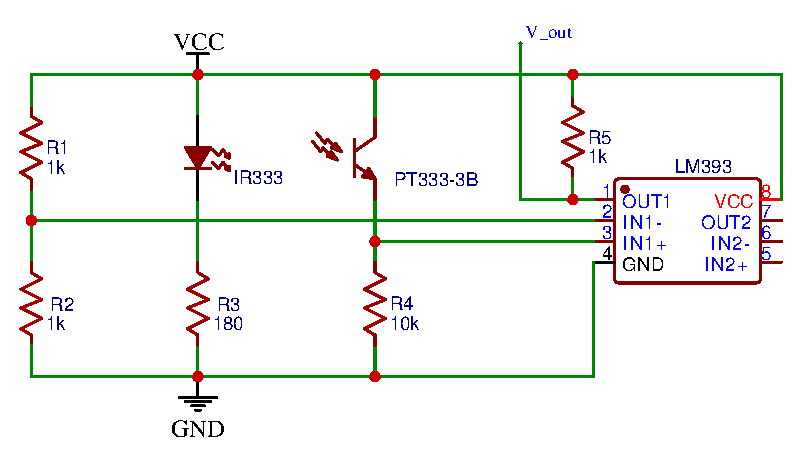
\includegraphics[scale=0.7]{figuras/Schematic_Sensor_barreira.pdf}
    \caption{Esquemático do circuito do sensor fotoelétrico de barreira}
    \label{fig:esq_sensor_barreira}
    \end{figure}
    
    \begin{itemize}
    \item[ ]
        \begin{itemize}
            \item 1 LED IR333;
            \item 1 Fototransistor PT333-3B;
            \item 1 CI LM393;
            \item 1 Resistor de 180 $\Omega$;
            \item 1 Resistor de 10 k$\Omega$;
            \item 3 Resistores de 1 k$\Omega$.
        \end{itemize}
    \end{itemize}
    
    Para realizar as simulações foi utilizado o Opto-acoplador \textbf{4N25}, no qual consiste em um CI que contém um LED emissor de infravermelho e um fototransistor NPN. Optou-se pela utilização desse componente na simulação, uma vez que, os valores de tensão e correte de entrada e saída são os mesmos para os componentes selecionados \textbf{IR333} e \textbf{PT333-3B}. Entretanto, a única variação do \textbf{4N25} em relação ao LED emissor \textbf{IR333} é a corrente de entrada de 50 $mA$ para o CI e 20 $mA$ para o LED, o que pode ser corrigido na simulação pela alteração do resistor do LED.
    
    Além do mais, foi adicionada uma sequência de pulsos na entrada do LED emissor para representar a passagem do objeto entre o emissor e o receptor. Já que com a passagem do objeto tem-se a ausência de luz e as junções inversamente polarizadas do fototransistor não conduzem corrente elétrica, resultando em uma resistência "infinita". Após a passagem do objeto tem-se novamente a incisão de luz nestas junções e sua resistência diminui, havendo assim a condução de corrente elétrica. 
    
    Tendo essa variação de corrente, tem-se também uma variação de tensão e dessa forma é possível utilizar o CI \textbf{LM393}, que contém dois amplificadores operacionais comparadores de tensão. Por conseguinte, liga-se a entrada inversora do comparador a um par de resistores cujos valores determinam a tensão de referência. Quando o valor na entrada não inversora for maior que o valor de referência na entrada inversora a saída do comparador tende a 5 V. Enquanto que, quando o valor na entrada não inversora for menor que o valor de referência na entrada inversora, a saída do comparador tende a 0V. 
    
    
    \begin{figure}[H]
    \centering
    \includegraphics[scale=0.65]{figuras/Sim_sensor_barreir_3.PDF}
    \caption{Simulação do Sensor Fotoelétrico de barreira}
    \label{fig:sim_sensor_barreira}
    \end{figure}
    
     Portanto, a partir dessa variação de tensão na saída pode-se detectar a passagem do objeto traduzindo a variação de 5V e 0V para uma representação digital ao ser conectado com a central de controle. Essa conexão utilizando 3 pinos: Terminal 1 é a alimentação do circuito em 5V, Terminal 2 é o terra (em inglês \textit{Ground} - GND) e o Terminal 3 é a saída do comparador \textbf{LM393}, representado como $V_{out}$ na o esquemático da figura \ref{fig:sim_sensor_barreira}. Como a saída $V_{out}$ é uma saída digital, ou seja, quando for 0V temos bit 0 e em 5V temos bit 1 não é necessária o uso de um condicionamento de sinal como conversores analógico digital para conexão entre o sensor desenvolvido e a central de controle.

    
    Por último, a partir da simulação foi realizada a placa de circuito impresso conforme a figura  \ref{fig:PCB_barreira} no apêndice \ref{app:PCB}.  
    

    Para levantamento da corrente total consumida pelo sensor de barreira é levado em consideração a corrente típica de operação para o \textit{LED} emissor ($I_{LED}$) e a corrente da fonte de alimentação para simulação na figura \ref{fig:sim_sensor_barreira} excluindo o IN25 ($I_{CIRCUITO}$). Como $I_{LED} = 20 mA $ e $I_{CIRCUITO} = 5mA$  obtemos a corrente total somando essa correntes. Ou seja, $I_{total} = I_{LED} + I_{CIRCUITO} = 25mA$.  

    % \item Sensor de Biometria
    \subparagraph*{$\bullet$ Sensor de Biometria} \hfill
    
    O sensor de biometria é utilizado para autenticação de usuários nos mais diversos produtos no mercado. O seu funcionamento se baseia na captura da digital do usuário por meio de uma imagem que posteriormente terá suas características únicas extraídas e comparadas com um banco de dados de digitais cadastradas. 
    
    Dessa forma foi escolhido o sensor óptico de digitais \textbf{DY50}, figura \ref{fig:sensor_biometria}, por ser o mais comum no mercado e possuir um sistema  validado para obtenção de digitais. Esse sensor tem a funcionalidade de legitimar o funcionário da clínica geriátrica e permitir realizar funções que necessitam de autenticação. Assim, esse sensor é empregado para liberar o compartimento frontal/traseiro para a retirada da dose medicamentosa do dispensador e realizar o abastecimento do estoque de medicamentos.
    
   A conexão do sensor com a central de controle consiste em 4 pinos, esquemático na figura \ref{fig:biometria_esq}: VCC e GND para alimentação, TX e RX para a comunicação UART. O sensor de biometria \textbf{DY50} está representado na figura \ref{fig:biometria_fig}, e possui as seguintes especificações:
    
    \begin{itemize}
    \item[ ]
        \begin{itemize}
            \item Alimentação: 3,6V a 6V;
            \item Consumo de corrente máximo: 120 $m$A;
            \item Taxa de transmissão : 9600, 19200, 28800, 38400, 57600 bps;
            \item Comunicação: TTL serial;
            \item Preço: R\$ 69,00.
        \end{itemize}
    \end{itemize} 
    
    \begin{figure}[H]
        \centering
        \subfloat[][Sensor DY50]{\includegraphics[width=0.3\textwidth]{figuras/sensor_biometria.jpg}\label{fig:biometria_fig}}
        \hspace{0.1\textwidth}
        \subfloat[][Conexões do Sensor DY50]{\includegraphics[width=0.3\textwidth]{figuras/esquematico_eletronica/esq_conex_biometria.png}\label{fig:biometria_esq}}
        \caption{Sensor Biometria DY50}\label{fig:sensor_biometria}
    \end{figure}
    
    % \item Sensor de Leitura RFID
    \subparagraph*{$\bullet$ Sensor de Leitura RFID} \hfill
    
    O sensor de identificação por radiofrequência (RFID) utiliza um sistema de energização sem fio de etiquetas RFID para obtenção de dados armazenados nelas. Dessa forma, é utilizada uma antena que realiza a energização e captação desses dados numa frequência de 13.56 MHz, que posteriormente são decodificados e enviados por meio do protocolo I$^2$C para central de controle. 
    
    O uso do sensor RFID foi pensado para identificar os copos utilizados para armazenar as doses de medicamentos. Desse modo, sua identificação é necessária para determinar o copo que está recebendo a medicação. Para realizar a identificação e logística de distribuição de medicamentos para os pacientes, cada copo tem cores únicas para evitar ministração de doses medicamentosas para pacientes errados. 
    
    Com o posicionamento da etiqueta RFID na parte inferior do copo é possível ler sua identificação independentemente da face virada para o sensor. Uma vez que o sensor será posicionado entre as placas da esteira e o sensor poder identificar etiquetas RFID com uma distância determinada dependendo da antena utilizada. Como as placas da esteira utilizada são feitas de plástico não ocorrerá problemas em relação a interferência na posição onde foi definido. 
    
    O modelo \textbf{PN532}, figura \ref{fig:sensor_RFID}, foi escolhido pela sua capacidade de distância de ativação das etiquetas chegar à 70mm e sua antena pode ser modificada e direcionada para atender as necessidades de dimensionamento da máquina.
    
    A conexão do sensor de leitura RFID com a central de controle consiste em 4 pinos, esquemático na figura \ref{fig:sensor_RFID_esq}: VCC, GND, SDA e SCL, que são duas linhas de dados para comunicação I$^2$C.
    
    \begin{itemize}
    \item[ ]
        \begin{itemize}
            \item Alimentação: 5V;
            \item Interfaces: I$^2$C, SPI e High Speed UART (HSU);
            \item Distância máxima de leitura/gravação: 7cm;
            \item Preço: R\$ 33,99.
        \end{itemize}
    \end{itemize}
    
\begin{figure}[H]
    \centering
    \subfloat[][Sensor de leitura RFID PN532]{
    \includegraphics[width=0.25\textwidth]{figuras/sensor_RFID.jpg}
    \label{fig:sensor_RFID}}
    \hspace{0.05\textwidth}
    \subfloat[][Conexões do módulo PN532]{
    \includegraphics[width=0.25\textwidth]{figuras/pinos_RFID.png}
    \label{fig:sensor_RFID_esq}}
    \caption{Módulo PN532}\label{fig:modulo_RFID}
\end{figure}
    
    O C.I. controlador RFID PN532 contempla um projeto de circuito com os componentes necessários para conectar uma antena, fornecido pelo fabricante. Este circuito RF consiste em 8 capacitores, 2 indutores, 2 resistores e a bobina de antena simétrica como mostrado na figura \ref{fig:antena_RFID}
    
    O filtro EMC reduz harmônicos de 13,56 MHz e executa uma impedância transformação. Em seguida, o circuito para casamento de impedâncias atua como um bloco de transformação de impedância. Por último, a própria bobina da antena gera o campo magnético, e assim recebe ou envia um sinal  correspondente processado pelo PN532.
    
    \begin{figure}[H]
    \centering
    \includegraphics[scale=0.7]{figuras/antena_RFID.png}
    \caption{Diagrama de blocos da parte RF}
    \label{fig:antena_RFID}
    \end{figure}

   Como foi escolhido um módulo do sensor de leitura RFID com o PN532 integrado, nele existe uma antena seguindo o projeto do fabricante. Essa antena suporta a distância de até 70mm para leitura e escrita em TAGs RFID compatíveis com a frequência de 13,56 MHz. Essa distância é suficiente para aplicação pois é superior a espessura do módulo da esteira utilizada, 19,9mm na figura \ref{fig:esteira} do apêndice \ref{cad_preliminar}.
   
   \subparagraph*{} $\bullet$ \textit{Tag} RFID \hfill
   
   Para escolha da tag RFID, primeiro deve ser observado se ela é para o tipo de frequência do sensor RFID utilizado, neste caso 13,56 Mhz. Em seguida, devemos ficar atentos para atender as dimensões e formato do copo utilizado. Pelas cotagens descritas na figura \ref{fig:copo} do apêndice \ref{cad_preliminar},  copo tem base com 55mm de diâmetro e 1,5mm de espessura. Por fim é necessário ser compatível com uma distância mínima de 50mm de leitura e escrita por variar dependendo do tamanho.
   
   Dessa forma foi escolhido a Tag etiqueta RFID 13,56 MHz, representado na figura \ref{fig:etiqueta_rfid}. Ela tem diâmetro de 25 mm, menor que a base do copo, e suporta uma distância de comunicação de 50 mm, suficiente para aplicação.

    \begin{figure}[H]
        \centering
        \includegraphics[width=0.3\textwidth]{figuras/etiqueta_rfid.jpg}
        \caption{Tag etiqueta RFID 13,56 Mhz}
        \label{fig:etiqueta_rfid}
     \end{figure}
%   Dessa forma, não será necessária a adição de uma outra antena para aumentar a distância de ativação das etiquetas, uma vez que, a antena embutida no módulo já contempla a distância necessária de 50mm para aplicação.
   
    % \item Câmera para Processamento de Imagens
    \subparagraph*{$\bullet$ Câmera para Processamento de Imagens} \hfill
    
    Atualmente câmeras estão presentes no dia-a-dia da população mundial, porém ainda mais presentes na automatização de processos industriais e verificação de qualidade por meio do processamento de imagens. Dessa forma, o uso de uma câmera foi escolhida para realizar a captação visual dos comprimidos. Posteriormente, a partir do  processamento dessas imagens, serão extraídas as características dos comprimidos, sendo possível identificar a quantidade e classificar o tipo de medicamento no copo de forma eficiente e confiável.
    
    A câmera escolhida foi a \textbf{OV5647}, figura \ref{fig:OV5647_pic}, por apresentar sensor com capacidade de gerar imagens de até 2592x1944 pixeis e preço acessível no Brasil. Ela utiliza o protocolo \textit{Camera Serial Interface} (CSI) para transmitir dados, sendo um padrão compatível para integração com a central de controle. Para realizar a conexão entre a câmera e a central de controle, especificamente o microprocessador utilizado, utilizamos um cabo \textit{flat} de 15 canais compatível com o soquete \textit{Zero Insertion Force} (ZIF) presente tanto no microprocessador como no módulo com a câmera OV5647, representação esquemática na figura \ref{fig:OV5647_esq},.
    
    \begin{figure}[H]
    \centering
    \subfloat[][Câmera OVN5647 com lente]{\includegraphics[width=0.25\textwidth]{figuras/OV5647.png}\label{fig:OV5647_pic}}
    \hspace{0.1\textwidth}
    \subfloat[][Conexões CSI da Câmera OVN5647]{
    \includegraphics[width=0.25\textwidth]{figuras/esquematico_eletronica/esq_conex_csi.png}\label{fig:OV5647_esq}}
    \caption{Câmera OV5647 - 5MP}\label{fig:camera_process}
    \end{figure}
    
    Para o processamento será aplicada uma técnica que consiste em detectar as bordas dos medicamentos. Com isso é criado máscaras binárias para cada comprimido identificado, isolando o comprimido e extraindo características do mesmo, como por exemplo, cor e formato.
    
    Após isso, será utilizado um classificador \textit{SVM}, treinado com uma biblioteca de imagens de comprimidos que tiveram as mesmas características extraídas. Sendo assim cruzados os dados dos comprimidos que eram previstos no copo com os dados do classificador SVM, obtendo resultado positivo caso seja verificado que a dose está correta. 
    
    O classificador \textit{SVM} foi escolhido por ter solução determinística, não possuindo viés de treinamento e não consumindo muitos recursos do sistema embarcado. 
% \end{itemize}

\section{Sistema de Acionamento de Atuadores}
     
    O sistema de acionamento de atuadores tem a funcionalidade de controlar os atuadores contidos no dispositivo. Sendo assim, o sistema de acionamento de atuadores  trata-se de um sistema micro-controlado pela central de controle e são utilizados \textit{drivers} que controlam os atuadores do dispositivo. Sendo estes: motor DC, atuador, motores de passo, solenoides para os contêineres e as mini travas elétricas solenóides em cada compartimento de acesso no sistema. 

% \begin{itemize}
%    \item Fechaduras
    % \item Drivers
    \subparagraph*{$\bullet$ Drivers} \hfill
    
    Os \textit{drivers} dos atuadores são módulos projetados para prover a potência de atuação e a interação com o controle de forma simplificada. Eles convertem comandos por meio de portas lógicas em potência controlada para os atuadores. Dessa forma, tornam possível o controle automático de ações de movimento.
    
    \subparagraph*{} $\bullet$ Motores de Passo
    
    O \textit{driver} escolhido para os motores de passo é o módulo com CI \textbf{A4988} pois atende as características de carga para funcionamento do motor de passo escolhido, explicado na seção \ref{energ:motor_passo} da solução energética, e inclui a possibilidade de resolução do passo do motor em até 1/16 do considerado passo completo pelo fabricante. Por não ser uma aplicação que necessite de alta resolução para controle dos motores de passo, por apenas girar os fusos que rotacionam as engrenagens de um grupo de 5 contêineres até ser detectado a queda de um medicamento, a resolução de 1/16 do passo completo do motor é suficiente para controle. 
    
    Para conexão entre a central de controle, especificamente o microcontrolador, e o \textit{driver} A4988 são utilizados 9 pinos:
    
    \begin{itemize}
        \item[ ]
        \begin{itemize}
            \item[ ]
            \begin{itemize}
                \item[$\bullet$] \textbf{VCC} e \textbf{GND} para alimentação da parte lógica
                \item[$\bullet$] \textbf{MS1}, \textbf{MS2} e \textbf{MS3} são as portas lógicas que determinam a resolução do Passo: Passo Completo (estado lógico: "000"); Meio Passo (estado lógico: "100"); 1/4 Passo (estado lógico: "010"); 1/8 Passo (estado lógico: "001");  1/16 Passo (estado lógico: "111").
                \item[$\bullet$] \textbf{\textit{ENABLE}} ativa (estado lógico: '1') ou desativa (estado lógico: '0') as saídas de tensão  e corrente para o motor de passo
                \item[$\bullet$] \textbf{\textit{DIR}} Determina a direção de rotação do motor.
                \item[$\bullet$] \textbf{\textit{STEP}} Entrada de controle principal que cada transição de '0' para '1' realiza o movimento conforme a resolução determinada pelas portas MSx.
                \item[$\bullet$] \textbf{$\overline{RESET}$} quando vai para o estado lógico '0' ele reseta o tradutor (bloco interno do CI que traduz as entradas de controle em tensões na saída para movimento do motor de passo) para um estado inicial pre determinado e desativa todas as portas de saída para os motores. Ele ignora todas as portas de entrada STEP até ele voltar para o estado lógico '1' (desativado).
            \end{itemize}
        \end{itemize}
    \end{itemize}
    
    \subparagraph*{} $\bullet$ Motor DC
    
    O \textit{driver} escolhido para o motor DC é o \textbf{L298N}, seu controle é baseado na ponte H. Ele atende as especificações elétricas para alimentação do motor DC escolhido, explicado na seção \ref{energ:motor_dc} da solução energética. A estrutura de ponte H de eletrônica de potência permite a manipulação da tensão da fonte no motor por meio de chaveamento, dessa forma, é possível controlar a velocidade do motor. Para o chaveamento será utilizado o controle por modulação de pulso (\textit{PWM}), presente no microcontrolador. Essa tecnologia varia o tempo de permanência do sinal lógico em baixo e alto, isso acarreta uma resposta que simula uma variação de intensidade de tensão, porém variando apenas o tempo que o sinal está ligado.  
    
    Para conexão entre a central de controle, especificamente o microcontrolador, e a ponte H L298 são utilizados 3 pinos:
    
    \begin{itemize}
        \item[ ]
        \begin{itemize}
            \item[ ]
            \begin{itemize}
                \item[$\bullet$] \textbf{IN1} e \textbf{IN2} (Entrada 1 e Entrada 2) são as entradas de controle do motor A na ponte H. São 4 possibilidades lógicas para esses pinos: "00" motor gira no sentido direto, "01" motor gira no sentido reverso, "10" freio do sentido direto e "01" freio do sentido reverso.
                \item[$\bullet$] \textbf{GND} para conectar as referências lógicas do microcontrolador e da ponte H.
            \end{itemize}
        \end{itemize}
    \end{itemize}
    
    Para conexão entre a central de controle, especificamente o microcontrolador, e o \textit{driver} A4988 são utilizados 9 pinos:
    
    \subparagraph*{} $\bullet$ Solenoides e Atuador Linear
    
    O \textit{driver} escolhido para as solenoides e o atuador linear o módulo com CI \textbf{IRF520N} pois atende as características elétricas para funcionamento deles, explicado nas seções \ref{energ:solenoide} e \ref{energ:atuador_linear} da solução energética. E suas configurações possibilitam a utilização de sinais PWM da porta lógica do microcontrolador para controle.
    
    
    % \item Isolamento
    \subparagraph*{$\bullet$ Isolamento} \hfill
    %% Escrever texto básico para usando optoacopladores
    
    A natureza dos atuadores gera ruídos de tensão e corrente que devem ser tratados, uma vez que, caso esse ruído chegue ao sistema de controle existe a possibilidade de causar mal funcionamento das funções de todos os circuitos presentes. Portanto, deve-se isolar o sistema de atuadores do sistema de controle. Para isso são utilizados opto-acopladores, que isolam o sistema transferindo sinais por meio de \textit{LEDs} emissores e receptores.
    
% \end{itemize}

\section{Central de Controle}

A central de controle é o sistema que irá realizar tanto a análise dos dados coletados no módulo de medição quanto o controle do sistema de atuadores do dispositivo. Bem como é por onde comandos são recebidos e enviados  no \textit{Backend} - nome que representa a parte da arquitetura de software que interage com a central de controle. 

O principal componente da central de controle é o microprocessador embarcado. Adicionalmente também temos aspectos funcionais para os usuários que interagem com o dispositivo. Esta interação é feita pelo subsistema denominado módulo de visualização.

% \begin{itemize}
%     \item Microprocessadores
    \subparagraph*{$\bullet$ Microprocessadores}  \hfill
    
    A adoção de microprocessadores é bastante comum atualmente em implementações de sistemas embarcados nas mais diversas aplicações. Em especial temos diversos fabricantes que implementaram sistemas usando microprocessadores que tem suporte a vários Sistemas Operacionais (SO) diferentes e incluem uma interface de entradas e saídas digitais com propósito geral, sendo denominadas como computadores de placa única (\textit{Single Board Computers} - SBCs). Alguns exemplos comuns no mercado são as placas \textit{Raspberry's Pi} desenvolvidas pela \textit{Raspberry Pi Foundation}, placas Tinker da ASUS, placas BeagleBoards da Texas Instruments e as placas NVIDIA Jetson da NVIDIA. 
    
    A utilização de uma \textit{SBC} é devido necessidade desse sistema desempenhar várias funções que necessitam do suporte de um computador com sistema operacional, realizando  operações para área eletrônica como: Processamento de imagens dos medicamentos; Interface gráfica do módulo de visualização; Captura de dados de múltiplos sensores; Controle dos atuadores.
    
    Também é necessário que o sistema utilizado tenha suporte a protocolos de comunicação I$^2$C, \textit{SPI}, \textit{UART} e \textit{CSI} entre o módulo de medição e visualização e a central de controle. Principalmente em conter pinos GPIO para realizar a conexão física desses protocolos. Além do mais, que o sistema operacional escolhido tenha suporte as ferramentas e algoritmos de comunicação com as arquiteturas usadas na área de Software.
    
    Após uma análise de vários modelos comparando principalmente os componentes integrados como processador central (CPU), processador gráfico (GPU), tipo de memória RAM, quantidade de memória RAM, periféricos embarcados (tipo USB, módulo Wi/Fi, internet) e o preço relativo praticado em fornecedores no Brasil foi escolhido a \textbf{Raspberry Pi 4 B} com \textbf{4GB DDR4}. 
    
    A Raspberry Pi 4 B tem suporte físico para os protocolos de comunicação suportados para comunicação entre os componentes da central de controle e sensores específicos do módulo de medição. Ou seja, em seu GPIO existem conexão da comunicação I$^2$C, \textit{SPI}, \textit{UART}, sendo que para o protocolo \textit{CSI} é utilizado o soquete ZIF de 15 pinos na parte traseira da placa. 
    
    Para o armazenamento será o tipo de armazenamento suportado em hardware pela Raspberry Pi 4, sendo o cartão de memória chamado em inglês de Secure Digital Card (SD Card). Para o tamanho do cartão de memória foi selecionado o de 32 Gb, por não ser realizado o armazenamento das imagens usadas no processamento de imagens e o banco de dados não armazenar volume de dados grande, apenas arquivos de Mbs e Kbs. Por fim, foi avaliado as especificações da velocidade de leitura e escrita do SD card em relação ao preço final. 
    
    Sendo assim, foi escolhido o SD Card \textbf{SanDisk Extreme} com \textbf{32GBs} de armazenamento e especificação de leitura em até 100 MB/s e escrita de 90 MB/s. Além de atender os requisitos, essa escolha foi baseada em um comparativo de velocidade realizado pela impressa especializada aliada ao preço em fornecedores locais \cite{sdcard_benchmark}. 
    
    Para o sistema operacional foi escolhido o Ubuntu Server 18.04.05 LTS por ser uma versão lançada a alguns anos no mercado (2018) e seu ciclo de vida terminar em Abril de 2023. O ciclo de vida representa o data fim em que a versão do sistema operacional para de receber suporte oficial da comunidade Ubuntu para atualizações de segurança e novidades. Esses sistema operacional suporta todos as bibliotecas utilizadas para desenvolvimento da comunicação e controle dos subsistemas da eletrônica como os utilizados pela solução de software.
    
    
    % \item Módulo de Visualização
    \subparagraph*{$\bullet$ Módulo de Visualização} \hfill
    
    O módulo de visualização é o subsistema onde o usuário poderá visualizar algumas informações úteis de funcionamento e gestão do dispositivo e interagir com essa interface usando as teclas de interação. Nele estão contidos um visor e um teclado para interface com o usuário.
    
    No presente ponto de controle apresenta-se no apêndice \ref{app_telas_display}  o \textit{mockup} desenvolvido para as telas presentes na interface.
    \newpage
    % \begin{itemize}
    %     \item Visor 
        \subparagraph*{}$\bullet$ Visor \hfill
        
        Existem diversas tecnologias de tela disponíveis no mercado que podem ser utilizadas no projeto. Para delimitação da tela foi levado em consideração compatibilidade do protocolo de comunicação com sistema microprocessado escolhido, tamanho da tela, tecnologia de tela para visualização nas cores RGB e preço relativo. Sendo assim foi escolhido a tela tipo LCD TFT de 3,2” com as seguintes características:
        
        \vspace{-0.2cm}
        \begin{itemize}
            \item[ ] 
            \begin{itemize}
            \item \textbf{\textit{Display}:} Tipo LCD TFT 3.2" 
            \item \textbf{Controlador:} ILI9341
            \item \textbf{Resolução:} 240x320 pixels
            \item \textbf{Dimensões da tela:} 48.60 x 64.80 mm
            \item \textbf{Interface:} SPI
            \end{itemize}
        \end{itemize}
        
        % \vspace{-0.2cm}
        
        \begin{figure}[H]
        \centering
        \subfloat[][Visor tipo LCD TFT]{\includegraphics[width=0.4\textwidth]{figuras/Display-LCD-TFT-3.2-240x320-6.jpg}\label{fig:LCD_pic}}
        \hspace{0.1\textwidth}
        \subfloat[][Conexões da tela LCD - Protocolo SPI]{
        \includegraphics[width=0.3\textwidth]{figuras/esquematico_eletronica/esq_lcd_320.png}\label{fig:LCD_esq}}
        \caption{Visor tipo LCD TFT 240x320}
        \label{fig:display_lcd}
        \end{figure}
        
        % \item Teclado
        \subparagraph*{}$\bullet$ Teclado \hfill
        
        A utilização de uma matriz de botões é necessária para o usuário do dispositivo poder interagir com os menus de opções disponíveis na tela de visualização. Neste caso foi preferível o uso de botões, uma vez que todos os cadastros de medicação, paciente, enfermeiro serão realizados pelo aplicativo e para utilizar menos processamento do sistema microprocessado. 
        
        
        Sendo assim será usado uma configuração de arquitetura chamada de matriz de botões, especificamente uma solução comercial \textit{AdKeypad} com 5 botões como foto na figura \ref{fig:keypad_ft}.
        
        \begin{figure}[H]
          \centering
          \begin{minipage}[b]{0.3\textwidth}
            \includegraphics[width=\textwidth]{figuras/adkeypad.jpg}
            \caption{\textit{AdKeypad} com 5 botões}
            \label{fig:keypad_ft}
          \end{minipage}
          \hspace{2cm}
          \begin{minipage}[b]{0.3\textwidth}
            \includegraphics[width=\textwidth]{figuras/adkeypad_schematic.png}
            \caption{Esquemático \textit{AdKeypad}}
            \label{fig:keypad_esq}
          \end{minipage}
        \end{figure}
        
        Analisando o circuito esquematizado na figura \ref{fig:keypad_esq} podemos calcular a saída de tensão do circuito dependendo do tipo de tecla que é clicada. O circuito se comporta como vários divisores de tensão, onde a resistência varia dependendo da tecla que é clicada. Assim obtemos a equação \ref{eq:teclado}, que representa o cálculo da tensão $V_{out}$ seguindo as entradas e saídas da figura \ref{fig:keypad_esq}.
        
        \begin{equation}\label{eq:teclado}
            V_{out} = \frac{R_{EQ}}{R_2 + R_{EQ}} \cdot 5 [V]
        \end{equation}
        
        Onde $R_2$ é o resistor de 2k$\Omega$ e $R_{EQ}$ é a soma dos resistores $R_8$, $R_7$, $R_6$ e $R5$ dependendo da tecla que está sendo clicada. Sendo assim temos o resultado de $V_{out}$ na tabela \ref{tab:teclado}.
        
        \begin{table}[H]
        \centering
        \caption{Resultado para tensão $V_{out}$}
        \label{tab:teclado}
        \begin{adjustbox}{max width = \textwidth}
            % \begin{tabular}{|L{5cm}|C{2cm}|C{2cm}|C{2cm}|C{2cm}|C{2cm}|}
            \begin{tabular}{|l|c|c|c|}
                \hline
                \rowcolor[HTML]{A8DADC}
                \textbf{Tecla} & $R_2$ [$\Omega$] & $R_{EQ}$ [$\Omega$] & $V_{out}$ [V] \\ \hline
                \textit{UP} & 2k & x & 0 \\ \hline
                \textit{DOWN} & 2k & 330  & 0,708 \\ \hline
                \textit{RIGHT} & 2k & 950 & 1,610 \\ \hline
                \textit{LEFT} & 2k & 1950 & 2,468 \\ \hline
                \textit{SELECT} & 2k & 5250 & 3,621 \\ \hline
                % Sensor de Temperatura e Umidade & 1	 & 3,3 & 0,0005 & 0,0015
            \end{tabular}
        \end{adjustbox}
        \end{table}
            
        
        Sua comunicação com microcontrolador é do tipo analógica, fazendo com o que o microcontrolador possua um conversor analógico digital para que seja realizada a leitura dos dados provenientes do teclado. Conforme o esquemático, na figura \ref{fig:keypad_esq}, pode-se observar que existe apenas um pino de dados (2) para esse teclado. Seu funcionamento se baseia em um circuito com várias divisões de tensão. A central de controle irá interpretar qual botão foi pressionado a partir do sinal digital resultante da conversão analógica digital da tensão de saída no pino de dados (2). Essa conversão é realizada em um microcontrolador, na qual o pino (2) de dados será conectado a uns dos pinos A/D de um dos microcontroladores que são usados no módulo de medição.
        
        
        
    % \end{itemize}
    
    % \item Microcontroladores
    \subparagraph*{$\bullet$ Microcontroladores} \hfill
    
    Os microcontroladores são utilizados nas mais diversas aplicações de controle e automação. Assim, os microcontroladores possuem os itens essenciais de processamento, aliados a periféricos abundantes para entradas e saídas de dados com um  baixo custo, possibilitam o desenvolvimento de sistemas robustos e escaláveis.
    
    % Melhor 
    Segundo John Morton \cite{morton2005pic}, para escolha do microcontrolador primeiro deve ser realizado um rascunho do projeto, observando o que será feito e o que o microcontrolador deve fazer. O próximo passo deve ser realizado um diagrama do circuito ou representação similar, vendo em particular todas as entradas e saídas necessárias para conectar com o microcontrolador atendem aos requisitos do projeto. Sendo um dos principais fatores de escolha devido a limitação de porta que cada microcontrolador tem. Como, por exemplo, PIC16F54 tem até 12 pinos entrada/saída (em inglês \textit{input/output} - I/O) e a PIC16F57 até 20.
    
    Dado a metologia de escolha, temos que em nosso projeto os microcontroladores serão utilizados para direcionar dados do módulo de medição para o sistema microprocessado e o mesmo enviar dados de controle para o sistema de acionamento de atuadores. Para direcionamento desses dados entre os microcontroladores e o sistema microprocessado escolhido (Raspberry Pi 4) foi determinado o uso do protocolo I$^2$C, sendo assim um requisito para escolha do microcontrolador.
    
    Para determinação da quantidade de pinos primeiro devemos listar a quantidade de cada componente conectado aos microcontroladores e os pinos necessários para cada unidade, excluindo pinos de alimentação como +5V e GND e observando se os pinos utilizados atendem a como o dado vem do sensor, ou seja, se é digital ou é necessário o uso de uma porta com conversão analógico-digital. Na tabela \ref{tab:pinos_microcontrolador} está a compilação da quantidade total de pinos necessários.
    
    \begin{table}[!htb]
    \centering
    \caption{Levantamento da quantidade de pinos}
    \label{tab:pinos_microcontrolador}
    \begin{adjustbox}{max width = \textwidth}
        \begin{tabular}{|L{5cm}|C{2cm}|C{2cm}|C{2cm}|C{2cm}|C{2cm}|}
            \hline
            \rowcolor[HTML]{A8DADC}
            \textbf{Componente} & \textbf{Quant. (unid.)} & \textbf{Pinos (Un)} &  \textbf{Tipo} & \textbf{Pinos (Total)}  \\ \hline
            % Sensor de Temperatura e Umidade & 1	 & 3,3 & 0,0005 & 0,0015
            % \\ \hline
           %   Sensor Fotoelétrico Emissor & 30	 & 3,3 & 0,1 & 9,9
         %   \\ \hline
              Sensor de Barreira & 30 & 1  & I/O & 30
             \\ \hline
             Interruptor Micro Switch & 30 & 1 & I/O & 30
            \\ \hline
             Teclado & 1 & 1 & Analógico & 1
            \\ \hline
            %  Cls Mux/Demux & 12 & 5 & 0,000001 & 
            % \\ \hline
               Driver A4988 & 5 & 7 & I/O & 35
             \\ \hline
               Driver IRF520N & 28 & 1 & I/O & 28
             \\ \hline
               Driver Ponte H L298 & 1 & 2 & I/O & 2
             \\ \hline
             \rowcolor[HTML]{F1FAEE}
             \multicolumn{4}{|l|}{\cellcolor[HTML]{F1FAEE}Total} & 126 \\
             \hline
        \end{tabular}
    \end{adjustbox}
\end{table}
    \subparagraph*{Nota:} Está sendo levado em consideração que a tela LCD, o sensor de biometria DY50, o sensor RFID PN532, o sensor de temperatura e umidade HTU21D e a câmera não se conectam aos microcontroladores.
    
    Analisando a tabela \ref{tab:pinos_microcontrolador} pode-se concluir que os componentes que contribuem para maior quantidade de pinos são os sensores de barreira, interruptores e \textit{driver} IRF520 para os solenoides/atuador linear. Como o uso de cada um desses componentes não é medido ou controlado paralelamente para aqueles que estão nos contêineres, 75 no total sendo 25 para cada tipo, o uso de multiplexadores e demultiplexadores é interessante por diminuir a quantidade de portas de I/O para conectar esse componentes com o microcontrolador. Sendo assim foi escolhido multiplexadores 8x1 e demultiplexador 8x1, especificamente pelo uso do CI CD4051. 
    
    O CD4051 é um CI de multiplexação ou demultiplexação com 13 pinos: São 8 pinos entradas/saídas; 1 pino saída/entrada; 3 pinos para chaveamento de qual dos 8 canais é a saídas; 1 pino \textit{ENABLE} que desliga o funcionamento do Ci. Dessa forma, a razão de redução de pinos conectados ao microcontrolador se agruparmos cada grupo de 25 componentes de tipos diferentes é de 11/24 utilizando 3 CD3051 para conectar 24 componentes e ligar um diretamente ao microcontrolador. Ou seja, diminuímos de 126 pinos para 52 a quantidade de pinos necessários. 
    
    Para evitar qualquer ruído inerente dos atuadores serão usados microcontroladores exclusivos tanto para o sistema de acionamento dos atuadores quanto para o módulo de medição. Desse modo, é garantida uma integridade dos valores medidos dos sensores no módulo de medição.
    
    Sendo assim, realizamos a separação dos pinos por tipo de sistema em que está conectado (módulo de medição ou sistema de acionamento de atuadores), componentes com maior quantidade (sensores barreira, interruptores e \textit{driver} IRF520N) e adicionando os pinos de conexão para o protocolo de comunicação I$^2$C (2 pinos - SDA e SCL) é necessário 4 microcontroladores com pelo menos 15 pinos. Onde um deles precisa ter uma entrada com conversor A/D para a conexão analógica do teclado. 
    
    Com a funcionalidade do microcontrolador determinada, da quantidade e tipo de pinos necessária e a quantidade de microcontroladores foi decidido usar os da família PIC, fabricados pela Microchip Technology. Sua arquitetura foi escolhida por ser compatível com bibliotecas de leitura, comunicação e controle dos \textit{drivers} dos atuadores. Também existe a disponibilidade em fornecedores locais de uma variedade de C.I.s de microcontroladores com diferentes quantidade de pinos I/O, conversão A/D de várias resolução e comunicação I$^2$. Sendo  possível a criação de circuitos customizados para aplicação sem a necessidade utilização de placas de desenvolvimento de microcontroladores, como Arduino UNO ou MSP430. Sendo assim, o microcontrolador escolhido foi o \textbf{PIC16F677} por conter 17 pinos I/O, onde 2 podem ser configurados para comunicação I$^2$C, 12 podem ser configurados como conversor A/D de 10 bits e pode ser alimentado com uma tensão de 5V, compatível com as duas possibilidades disponíveis pela solução energética.
    
% \end{itemize}
\section{Protocolos de comunicação}
\subsection{Protocolos internos}

Os protocolos internos são aqueles utilizados para comunicação entre os subsistemas e componentes da solução eletrônica.

\begin{itemize}
    \item I$^2$C
    
    O protocolo I$^2$C descreve o funcionamento de um barramento serial que opera com dois fios, SCL que é responsável por levar o clock do dispositivo mestre para os dispositivos escravos e o SDA para a transferência de dados. Para iniciar uma comunicação com escravos, o mestre coloca o valor lógico da linha SDA em baixo, logo em seguida é enviado o endereço do escravo que será utilizado. 
    
    Se o dispositivo escravo existir naquele endereço, um sinal de nível baixo é enviado pelo canal SCL após o oitavo pulso de clock. Após isso, o mestre lê ou escreve nos registradores selecionados do escravo. Ou seja, é uma comunicação bidirecional. 
    
    Na aplicação proposta este protocolo é usado para comunicação do dispositivo mestre, sistema microprocessado (Raspberry Pi 4), com dispositivos escravos. Os escravos são os quatro microcontroladores PIC16F677, o sensor de temperatura/umidade e o sensor RFID. 
    \newpage
    \item SPI
    
    O protocolo SPI possui 3 fios fixos e mais um para cada escravo no sistema. Sua comunicação é unidirecional em cada fio de comunicação, sendo o MOSI (Master Output Slave Input) partindo do mestre para o escravo, o MISO (Master Input Slave Output) partindo do escravo para o mestre, e o SCLK que é o clock serial do mestre. Para controlar qual escravo está sendo usado, é utilizado o pino de seleção de escravo SS, que precisa de um nível baixo para operar. Por mais que este protocolo precise de mais canais para seu funcionamento, as velocidades alcançadas  superam as do I$^2$C pois a deformação do sinal é menor pelo uso de transistores definindo o estado do pino (Push-Pull) ao invés de dreno aberto (Pull-Up).
    
    O protocolo SPI é utilizado para comunicar o dispositivo mestre, sistema microprocessado, com a tela LCD TFT 240x320. Devido a ser o protocolo compatível com o controlador da tela escolhida.
    
    
    \item UART
    
    O protocolo UART utiliza dois canais de comunicação, o RX que recebe dados e o TX que envia. Esse protocolo trabalha de forma assíncrona, necessitando de que o transmissor e receptor estejam numa mesma taxa de transmissão (em inglês \textit{baudrate}).
    
    As conexões são feitas invertendo-se os canais em dois dispositivos distintos, ou seja, o canal TX é conectado no RX e vice-versa. Para iniciar uma transmissão é enviado um bit de início, seguido de 5 a 9 bits de informação, um bit de paridade e um a dois bits de finalização de transmissão.
    
    Este protocolo é usado para comunicar o dispositivo mestre, sistema microprocessado, com o sensor de biometria DY50. 
    
    \item CSI
    
    O protocolo CSI (Camera Serial Interface) é caracterizado por uma fusão entre os protocolos I$^2$C e SPI. Ele utiliza duas interfaces, a primeira com os canais SCL e SDA para controle da câmera e a segunda com um canal de transmissão unidirecional da câmera para o processador e um canal de clock da câmera para o processador.
    
    Este protocolo é o utilizado para comunicação entre a Raspberry Pi 4 e o módulo com câmera OV5647.
    
    
    
\end{itemize}
\subsection{Protocolos externos}

Os protocolos externos são aqueles utilizados para comunicação entre os sistemas de controle e alimentação do dispositivo com o \textit{backend} da solução de software, esse é melhor detalhado \ref{sec:software_backend}.

\begin{itemize}
    \item HTTP
    
    O protocolo HTTP será utilizado para requisições de dados do sistema embarcado para o \textit{backend}. As informações requisitadas serão relacionadas a dados de funcionamento do sistema, como horários de medicação e dados de posicionamento dos medicamentos no sistema. Logo será uma comunicação unidirecional feita do sistema embarcado para o \textit{backend}.
    
    \item MQTT
    
    O protocolo MQTT será utilizado para comandos e confirmações, dessa forma é possível realizar requisições do \textit{backend} para ações na máquina, como cadastro de enfermeiros ou reposição de remédios. Portanto existem  tópicos dedicados a enviar confirmações de que as ações requisitadas foram realizadas e atualizações de dados da máquina para o \textit{backend}.
    
    
\end{itemize}

\section{Diagramas Esquemáticos da Conexão dos Sistemas}\label{sec:esq_conec_sistemas}

Os diagramas esquemáticos da conexão entre os componentes dos sistemas da solução eletrônica se encontram detalhados nos Esquemáticos Eletrônicos no apêndice \ref{esquematicos_eletronica}.

\section{Arquitetura de Eletrônica}

No diagrama lógico da arquitetura geral da eletrônica na imagem \ref{fig:fluxograma_eletronica} tem-se a interação dos módulos de medição com a central de controle e a interação do sistema de acionamento dos atuadores com a central de controle. Essa comunicação interna do dispositivo está explicada e esquematizada no apêndice \ref{esquematicos_eletronica}. Além do mais, nesse fluxograma é apresentada a alimentação necessária para cada componente.


\begin{figure}[H]
    \centering
    % \begin{adjustbox}{max width = \textwidth}
    \includegraphics[width=1.1\textwidth]{figuras/fluxograma_eletronica.png}
    \caption{Diagrama Lógico Eletrônico}
    \label{fig:fluxograma_eletronica}
    % \end{adjustbox}
\end{figure}



\section{Rede de Petri}

A Rede de Petri é uma técnica de modelagem, a qual permite a representação de sistemas com embasamento matemático, e assim relaciona causa e efeito entre os eventos e as condições. Os elementos básicos que formam a topologia da redes de Petri são:
\begin{itemize}
    \item \textbf{Estados:} são usados para modelar os componentes passivos dos sistemas, correspondendo às variáveis de estado, no diagrama são representadas por retângulos.
    \item \textbf{Ações:} são usadas para modelar os componentes ativos dos sistemas, são
    os eventos de transição de um estado para outro, no diagrama são representadas por círculos.
    \item \textbf{Fluxo:} através das ações do sistema é especificado como é a transformação de um estado para outro, no diagrama são representados por setas.
\end{itemize}

Para representar e modelar o controle do dispositivo utiliza-se a Rede de Petri. Antes de iniciar o processo de controle os medicamentos são retirados das embalagens e são posicionados nos contêineres. Além do mais, os copos esterilizados também são dispostos no local de armazenamento dentro do dispositivo. A partir da Rede de Petri, na figura \ref{fig:rede_petri},  percebe-se que ocorrem dois processos em paralelo a separação do medicamento e o posicionamento do copo na esteira. 

O primeiro processo tem início com o medicamento sólido no contêiner, no qual cai na comporta com a ativação do \textit{driver} do motor de passo. O medicamento é detectado pelo sensor fotoelétrico de barreira e, em seguida, deve-se desativar o drive do motor de passo quando ocorre a detecção para que não caia mais de um medicamento na comporta. Posteriormente, o solenoide é ativado para abrir a comporta. Quando a comporta é aberta o medicamento se desloca pelo canal de distribuição e, consequentemente, o solenoide é desativado. Em seguida, logo no final do funil do canal de distribuição, existe um sensor fotoelétrico de barreira para detectar a passagem do medicamento. Entretanto, quando o medicamento não é detectado pelo sensor, tem-se um aviso na tela do dispositivo que o medicamento está preso no dispositivo.

Enquanto isso, o outro processo em paralelo tem início com o copo no local de armazenamento. Sendo assim, no final do depósito de copos está posicionado um sensor de barreira para verificar e detectar a passagem do copo. Logo quando o copo é detectado deve-se ativar o \textit{driver} do atuador. Em seguida, quando o atuador é ativado, o copo é empurrado para a esteira e o \textit{driver} do atuador é desativado. Quando o copo está na esteira, é realizada a leitura da etiqueta RFID e os medicamentos são dispostos no copo a partir do posicionamento do copo abaixo do funil. Em uma dose medicamentosa que envolva mais de um comprimido o copo fica esperando até atingir o final do processo de separação dos medicamentos.

Posteriormente, quando ocorre a queda de todos os medicamentos da dose individual do paciente, o \textit{driver} da esteira é ativado e ela rotaciona para o sentido horário. Sendo assim, quando o copo com os medicamentos é detectado por outro sensor fotoelétrico de barreira, o qual é posicionado logo abaixo da câmera, o \textit{driver} da esteira é desativado e a esteira para. Com a finalidade de realizar o captura das imagens para o processamento de imagem. 

Quando o processamento de imagens da dose individual conclui que existe erros de quantidade ou seleção, a esteira é ativada com o movimento anti-horário até chegar em outro sensor de barreira. Esse sensor detecta que o copo com medicamento caiu no compartimento de doses medicamentosas erradas. Caso contrário, quando a quantidade e a seleção de medicamentos estão corretas, a esteira é ativada com o movimento horário até chegar sensor de barreira que detecta que o copo está na zona de entrega e que o medicamento foi retirado do dispositivo. 

Portanto, quando existe um horário que mais de um paciente necessita da administração da medicação, a dose de medicamentos individuais é realizada sequencialmente para cada paciente. Quando é detectado que o copo está na zona de entrega o dispositivo retorna para a posição inicial para a nova sequência de dose individual.

No processo de reabastecimento, em que é necessário abrir a comporta superior para adição de medicamentos e retirar os contêineres para limpeza, utiliza-se um interruptor. Com ele é possível detectar se a porta está fechada e se os contêineres estão corretamente encaixados. Caso contrário, deve-se enviar um aviso na tela para que o enfermeiro possa corrigir essas anomalias. 

\begin{figure}[H]
    \centering
    \includegraphics[width=1.4\textwidth, angle = -90]{figuras/petri.pdf}
    \caption{Rede de Petri do Controle eletrônico}
    \label{fig:rede_petri}
\end{figure}

\section{Processamento de Imagens}

A partir do  processamento de imagens é possível identificar a quantidade e classificar o tipo de medicamento no copo. Dessa forma, o processamento de imagens é um método para verificação se a dose medicamentosa que vai ser entregue ao paciente está correta conforme a receita médica.

\subsection{Separação dos comprimidos}

A primeira etapa para extrair dados da imagem é isolar os comprimidos presentes. Para isso é preciso a conversão da imagem para escala de cinza, facilitando assim na utilização de operações de filtragem na imagem em etapas subsequentes. Para exemplificar a explicação daqui em diante utiliza-se uma imagem do banco de dados, original na Fig. \ref{fig:proOrig}, e aplicando a conversão para escala de cinza temos o resultado na Fig. \ref{fig:proCinza}.

Em seguida, é necessária a detecção das bordas do comprimido. Como as imagens do banco de dados possuem um fundo padronizado o uso da técnica de limiar é possível. Um resultado possível pode ser observado na Fig. \ref{fig:proLim}. 

O próximo passo é eliminar resíduos da imagem deixando apenas o contorno do comprimido. Para isso são realizadas operações de abertura e fechamento utilizando elementos estruturantes circulares maiores que o resíduo e menores que o comprimido. Com isso obtemos uma máscara do exemplo utilizado, na Fig. \ref{fig:proMask}.

Por fim, uma técnica de detecção de objetos conectados é aplicada, a qual consegue separar objetos na imagem por meio de observação da vizinhança na imagem. Aplicando essa técnica nos exemplos temos o resultado nas Fig. \ref{fig:proMask1} e \ref{fig:proMask2}.

Com a máscara segmentada é possível separar os comprimidos por meio de uma multiplicação com a imagem original, com isso obtemos as Fig. \ref{fig:proPill1} e \ref{fig:proPill2}.

\begin{figure}[H]
        \centering
        \subfloat[][Original]{\includegraphics[width=0.3\textwidth]{figuras/eletronica/processamento/original.jpg}\label{fig:proOrig}}
        %\hspace{0.1\textwidth}
        \subfloat[][Escala de cinza]{
        \includegraphics[width=0.3\textwidth]{figuras/eletronica/processamento/cinza.jpg}\label{fig:proCinza}}
        \subfloat[][Limiar]{
        \includegraphics[width=0.3\textwidth]{figuras/eletronica/processamento/limiar.jpg}\label{fig:proLim}}
        
        \subfloat[][Máscara]{
        \includegraphics[width=0.3\textwidth]{figuras/eletronica/processamento/mascara.jpg}\label{fig:proMask}}
        \subfloat[][Objeto 1]{
        \includegraphics[width=0.3\textwidth]{figuras/eletronica/processamento/mascara1.jpg}\label{fig:proMask1}}
        \subfloat[][Objeto 2]{
        \includegraphics[width=0.3\textwidth]{figuras/eletronica/processamento/mascara2.jpg}\label{fig:proMask2}}
        
        \subfloat[][Comprimido 1]{
        \includegraphics[width=0.3\textwidth]{figuras/eletronica/processamento/pilula1.jpg}\label{fig:proPill1}}
        \subfloat[][Comprimido 2]{
        \includegraphics[width=0.3\textwidth]{figuras/eletronica/processamento/pilula2.jpg}\label{fig:proPill2}}
        
        \caption{Processo de separação}
        \label{fig:proCond}
\end{figure}

\subsection{Extração de características}

Com os comprimidos separados é possível extrair informações que serão utilizadas para classificá-los.

\begin{itemize}
    \item \textbf{Cor}
    
    Para extrair a cor do comprimido será utilizada uma média de cor de toda a região, eliminando possíveis efeitos de sombra presentes. Sendo assim, serão estabelecidos rótulos que corresponderão a uma faixa específica do espectro RGB das imagens.
    
    \newpage
    \item \textbf{Formato}
    
    Para extrair o formato do comprimido será utilizada a técnica de \textit{template matching}. Ela consiste em comparar a imagem com modelos pré-definidos, realizando a correlação da imagem com o \textit{template}. Se a correlação for próxima de 1, significa que há uma alta probabilidade do formato estar correto. Consequentemente, é possível testar todos os formatos possíveis e identificar qual a maior correlação entre eles.
    
    \item \textbf{Texto estampado}
    
    Para extrair o texto do comprimido é necessário o tratamento da imagem para que os contornos sejam destacados, com isso obteremos a Fig. \ref{fig:propilLim}, porém o objeto de texto ainda possui áreas não conectadas. Para contornar esse problema é utilizado uma abertura na imagem com um objeto estruturante circular pequeno com até 5 pixeis de diâmetro. Assim obtemos como resultado uma melhor definição das letras, mostrado na Fig. \ref{fig:propilAb}.
    
    Por fim, subtrai-se a máscara do comprimido do resultado anteriormente obtido e, consequentemente, no isolamento do texto a ser processado. O resultado da subtração da máscara pode ser visualizado na Fig. \ref{fig:propiltext}.
    
    Para interpretar o texto será utilizado o \textbf{Tesseract}, um sistema de reconhecimento óptico de caracteres (OCR), o qual utiliza uma rede neural treinada para identificar linhas de texto. Para utilização desse sistema é necessário identificar a região de interesse e isolá-la para melhores resultados. Assim obtemos o resultado na Fig. \ref{fig:propiltextex}, onde é possível observar a região de interesse que possui texto e o valor reconhecido.
    
    \begin{figure}[H]
        \centering
        \subfloat[][Destaque dos contornos]{\includegraphics[width=0.3\textwidth]{figuras/eletronica/processamento/pilulalimiar.jpg}\label{fig:propilLim}}
        \hspace{0.05cm}
        \subfloat[][Conexão das letras]{\includegraphics[width=0.3\textwidth]{figuras/eletronica/processamento/pilulaabertura.jpg}\label{fig:propilAb}}
        \hspace{0.05cm}
        \subfloat[][Texto isolado]{\includegraphics[width=0.3\textwidth]{figuras/eletronica/processamento/texto.jpg}\label{fig:propiltext}}
        
        \subfloat[][Texto identificado]{\includegraphics[width=0.4\textwidth]{figuras/eletronica/processamento/textoExtraido.png}\label{fig:propiltextex}}
        
        
        \caption{Extração de texto}
        \label{fig:proText}
    \end{figure}
\end{itemize}

\subsection{Máquina de Vetores de Suporte (SVM)}

Para conseguir identificar diversos comprimidos nas imagens é necessário o uso de um classificador. Existem diversos tipos de classificadores e o escolhido foi a máquina de vetores de suporte (SVM). 

Seu funcionamento se baseia na ideia de gerar uma superfície que separa as classificações por meio das características empregadas. Dessa forma, para realizar o o treinamento da SVM são criados vetores de suporte que separam a área entre classificações.

Assim, para o treinamento será utilizado um banco de imagens de comprimidos feito pela \textit{National Library of Medicine} que possui 4 mil imagens em ambiente controlado e 133 mil em imagens amadoras, o banco de imagens está disponível no  \href{https://www.nlm.nih.gov/databases/download/data_distrib_main.html}{link}. 

O tipo de classificação utilizada será a `\textit{yes or no}', na qual serão criadas SVMs para cada comprimido a ser identificado e deve-se ensinar como identificar características individuais dos comprimidos.



\section{Plano de Construção}

Para construção dos subsistemas da eletrônica foi pensado levando em consideração os esquemáticos descrição na seção \ref{sec:esq_conec_sistemas}. Desses esquemáticos pode ser gerado as placas de circuito impresso, que serve como base para conexão de todos subsistemas e seus componentes da área eletrônica. 

Para o projeto das PCI foi utilizado o software \textit{Proteus} utilizando placas de fibra de vidro de camada dupla. Em alguns casos a camada oposta possui vias passantes para realizar conexões. Foram utilizadas somente angulações de 45 e 60 graus para as vias roteadas em todos os layouts. E também, não existir a inversão da conexão dos pinos conectados, foram utilizados conectores Molex KK e uma legenda em cada PCB para os conectores. As figuras no apêndice \ref{app:PCB} mostram os \textit{layouts} para as placas fabricadas. Ademais, em todos os casos foram utilizadas zonas preenchidas de Ground (GND) na camada de cobre.

\subsection{Central de Controle}

A PCI do sistema central, figura \ref{fig:PCB_central}, foi criada para funcionar como um \textit{shield} para a Raspberry Pi4. Ou seja, a barra de pinos fêmea 2x20 dessa PCI se conecta com a GPIO da Raspberry Pi 4. Na parte superior é conectado:

\begin{itemize}
    \item Fonte de alimentação 5V/8A: Cabo com conector Molex KK de 2 pinos fêmea/fêmea;
    \item LCD 240x320: Cabo com conector Molex KK de 8 pinos fêmea/fêmea;
    \item Quatro PCBs que contêm os microcontroladores: 4 Cabos com conector Molex KK de 4 fêmea/fêmea;
    \item Sensor Temperatura e Umidade HTU21D: Cabo com conector Molex KK de 4 pinos fêmea/fêmea;
    \item Sensor RFID PN532: Cabo com conector Molex KK de 4 pinos;
    \item Sensor de Biometria: Cabo com conector Molex KK de 6 pinos;
\end{itemize}

Para conectar a câmera OV5647 com a Raspberry é utilizado um cabo \textit{flat} de 15 canais com 300mm de comprimento. 

\subsection{Módulo de Medição}

Para o módulo de medição são utilizados duas placas PCI, representadas no esquemático 1 na figura \ref{fig:esquematico_1}, como a PIC16 1 e PIC16 2.

Para a PCI especificada para PI16 1, figura \ref{fig:PCB_micro1}, ocorre as seguintes conexões:

\begin{itemize}
    \item[]
    \begin{itemize}
    \item Conexão com a PCI central: Cabo com conexão Molex KK de 4 pinos fêmea/fêmea que foi conectado no conector de legenda PIC16 1 na PCI central.
    \item 30 Sensores de Barreira: 30 Cabos com conexão Molex KK de 2 pinos fêmea/fêmea com a outra ponta conectada as 30 PCIs representadas na figura \ref{fig:PCB_barreira}.
\end{itemize}
    
\end{itemize}


Para a PCI do sensor de barreira, figura \ref{fig:PCB_barreira}, além de ser conectado o cabo vindo a PCI PIC16, devemos utilizar 2 cabos adicionais com 2 terminais cada para conectar o PT333-3B e IR333 para cada sensor. 

Para a PCI especificada para PI16 2, figura \ref{fig:PCB_micro2}, ocorre as seguintes conexões:

\begin{itemize}
    \item[]
    \begin{itemize}
    \item Conexão com a PCI central: Cabo com conexão Molex KK de 4 pinos fêmea/fêmea que foi conectado no conector de legenda PIC16 2 na PCI central.
    \item 30 Interruptores: 30 Cabos com conexão Molex KK de 2 pinos fêmea/fêmea com a outra ponta conectada aos interruptores no terminal Comum e Normal Fechado (Pino 1 e Pino 2).
    \item Teclado: Cabo com conexão Molex KK de 3 pinos fêmea/fêmea
\end{itemize}
\end{itemize}


\subsection{Módulo de Acionamento dos Atuadores}

Para o módulo de acionamento dos atuadores são utilizados duas placas PCI, representadas no esquemático 1 na figura \ref{fig:esquematico_1}, como a PIC16 3 e PIC16 4.

Para a PCI especificada para PI16 3, figura \ref{fig:PCB_micro3}, ocorre as seguintes conexões:

\begin{itemize}
    \item[]
    \begin{itemize}
    \item Conexão com a PCI central: Cabo com conexão Molex KK de 4 pinos fêmea/fêmea que foi conectado no conector de legenda PIC16 3 na PCI central.
    \item 28 \textit{drivers} IRF520N: 28 Cabos com conexão Molex KK de 2 pinos fêmea/fêmea com a outra ponta conectada aos pinos de sinal e GND do \textit{driver} IRF520N.
\end{itemize}
\end{itemize}


Para a PCI especificada para PI16 4, figura \ref{fig:PCB_micro4}, ocorre as seguintes conexões:

\begin{itemize}
    \item[]
    \begin{itemize}
    \item Conexão com a PCI central: Cabo com conexão Molex KK de 4 pinos fêmea/fêmea que foi conectado no conector de legenda PIC16 4 na PCI central.
    \item 5 \textit{drivers} A4988:  Cabo com conexão Molex de 9 pinos fêmea/fêmea
    \item \textit{Driver} L298: Cabo com conexão Molex de 3 pinos fêmea/fêmea
\end{itemize}
\end{itemize}


%\ref{fig:PCB_barreira}
%\ref{fig:PCB_central}
%\ref{fig:PCB_micro1}
%\ref{fig:PCB_micro2}
%\ref{fig:PCB_micro3}
%\ref{fig:PCB_micro4}